\documentclass[11pt,letterpaper]{article}
\usepackage[margin=1in]{geometry}
\usepackage{graphicx}
\usepackage{hyperref}
\usepackage{listings}
\usepackage{amsmath}
\pagestyle{headings}
\usepackage{epstopdf}

\begin{document}

\title{PHY 410 \\ Homework Assignment 6}
\author{Han Wen \\ \tiny Person No. 50096432}
\date{\today}

\maketitle

\begin{abstract}
The goal of this assignment was to get familiar with the non-linear analysis, including finding minima and maxima for multiple dimension functions, and its application on models of NaCl.


\end{abstract}

\tableofcontents

\newpage
\section{Problem 1}

\subsection{Description}

Now consider the 2-d function:
$$
V(x,y)=-\frac{1}{2}r^2+\frac{1}{4}r^4
$$
where:
$$
r=\sqrt{x^2+y^2}
$$

Try to minimize this function with the BFGS algorithm for various x,y values. What can you observe about the behavior? How many maxima are there? How many minima? 

\subsection{Numerical Analysis}

To better evaluate its maxima and minima, I plotted the function with WolframAlpha interface \cite{plot of 2d function} ~\ref{figure1}. We can see it has a "ring" of minima and one local maxima, when x,y approach infinite the function goes to infinite as well.
Using the program to find the minima, with various initial guess of x and y (and the same accuracy 0.0000001)is shown in the table: \ref{table1}

\begin{figure}
\begin{center}
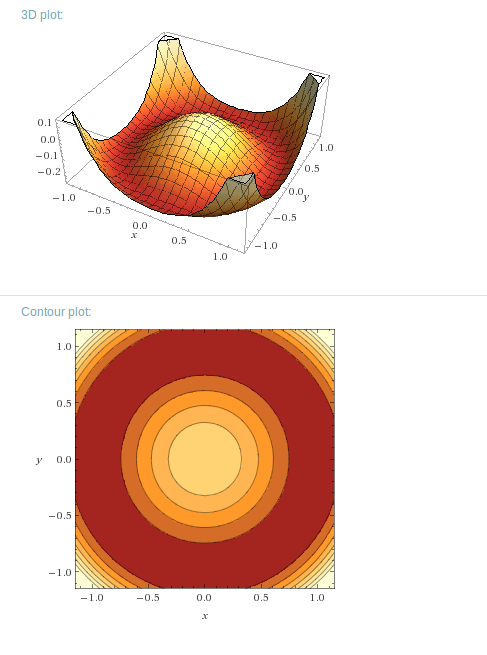
\includegraphics[width=0.8\linewidth,angle=0]{p1.png}
\caption{diagram of the function}
\label{figure1}
\end{center}
\end{figure}


\begin{table}[h]
\caption{trials\label{table1}}
\begin{tabular}{l l l l l}
\hline
 \textbf{initial x } & \textbf{initial y} & \textbf{iterations} & \textbf{final x}& \textbf{final y}\\
\hline
0.1 & 0.1 & 4 & 0.7071 & 0.7071 \\
1.5 & 1 & 4 & -0.8321 & -0.5547 \\
1 & 1.5 & 4 & -0.5547 & -0.8321 \\
5 & 1 & 8 & -0.9806 & -0.1961 \\
3 & 4 & 5 & -0.6 & -0.8 \\
\hline
\end{tabular}
\end{table}
From the table we can find that for the x and y we input, the final out put will be proportional to the input with $x^2+y^2=1$. 

\newpage

\section{Problem 2}

\subsection{Description}
  Determine the equilibrium configurations of NaCl clusters for  n=3 and n=4. Plot them using the macros from class (x,y,z in scatter plots). To find all of the equilibrium configurations, use the strategy we talked about in class to determine all of the local minima. You can look at this paper for inspiration of how to find the correct configurations : K. Michaelian, "Evolving few-ion clusters of Na and Cl",Am. J. Phys. 66, 231 (1998). \cite{paper}

\subsection{Result}
To find the all the configurations, I used the random initial positions, yet due to the precision problem, I believe it's better I use this method to first generate lots of final minimized configurations, then pick the different configurations out of them, then set those configurations as input to better evaluate the minimized energy and coordinates. 

For $Na_3Cl_3$, I found two different configurations:\\

First one ~\ref{figure2}, with binding energy -6.824eV\\


\begin{figure}
\begin{center}
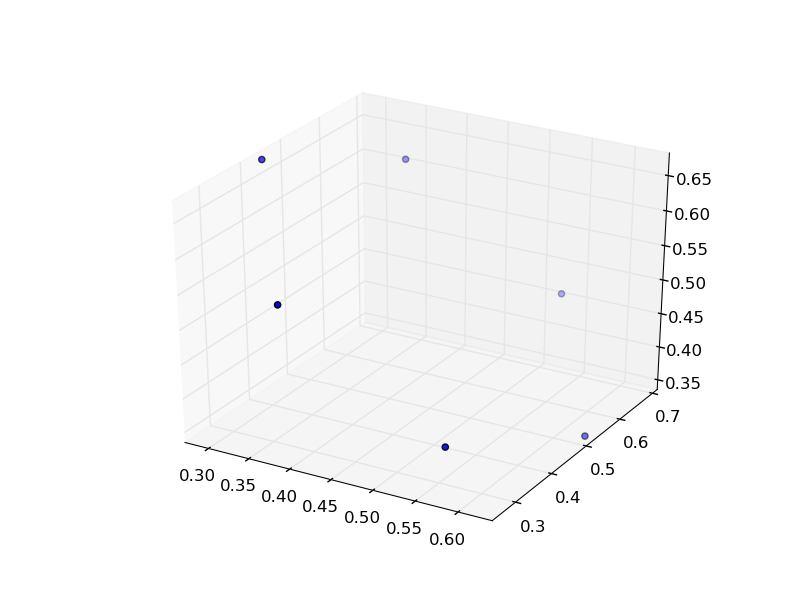
\includegraphics[width=0.8\linewidth,angle=0]{na3_1.png}
\caption{$Na_3Cl_3$ first configuration}
\label{figure2}
\end{center}
\end{figure}

Second one ~\ref{figure3}, with binding energy -6.382eV\\

\begin{figure}
\begin{center}
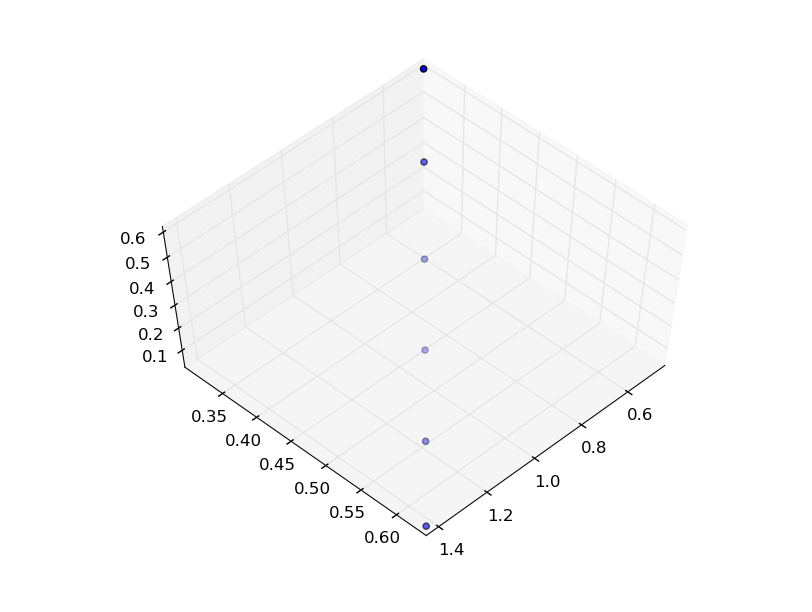
\includegraphics[width=0.8\linewidth,angle=0]{na3_2.png}
\caption{$Na_3Cl_3$ second configuration}
\label{figure3}
\end{center}
\end{figure}

For $Na_4Cl_4$, I found two different configurations:\\
First one ~\ref{figure4}, with binding energy -7.066eV

\begin{figure}
\begin{center}
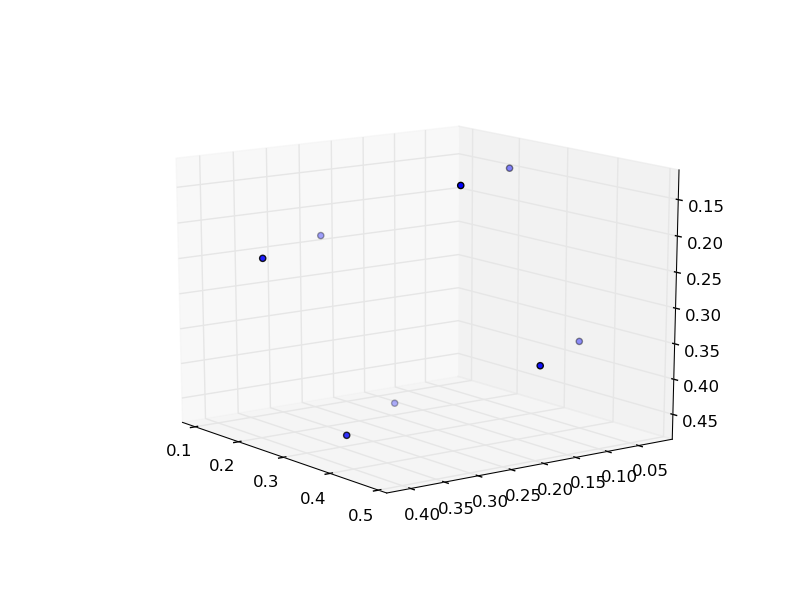
\includegraphics[width=0.8\linewidth,angle=0]{na4_1.png}
\caption{$Na_4Cl_4$ first configuration}
\label{figure4}
\end{center}
\end{figure}


Second one ~\ref{figure5}, with binding energy -6.957eV

\begin{figure}
\begin{center}
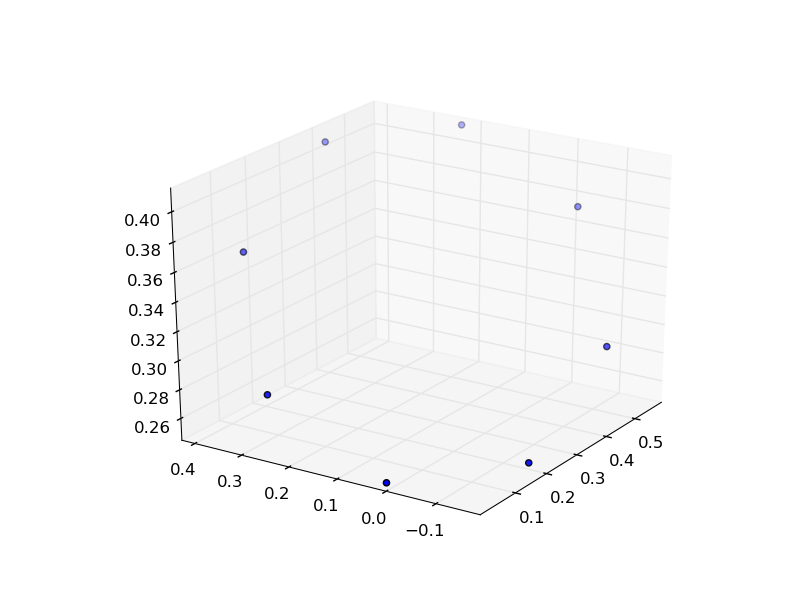
\includegraphics[width=0.8\linewidth,angle=0]{na4_2.png}
\caption{$Na_4Cl_4$ second configuration}
\label{figure5}
\end{center}
\end{figure}

Third one ~\ref{figure6}, with binding energy -6.933eV

\begin{figure}
\begin{center}
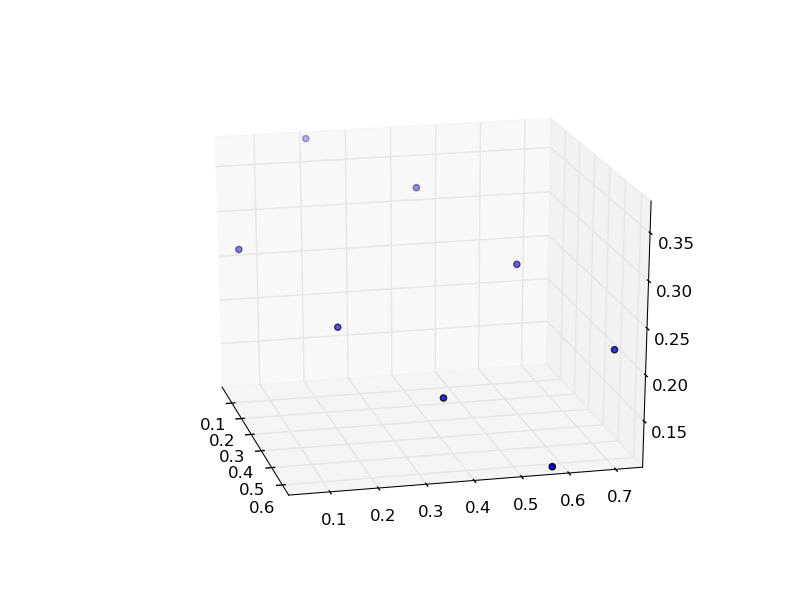
\includegraphics[width=0.8\linewidth,angle=0]{na4_3.png}
\caption{$Na_4Cl_4$ third configuration}
\label{figure6}
\end{center}
\end{figure}

Fourth one ~\ref{figure7}, with binding energy -6.847eV

\begin{figure}
\begin{center}
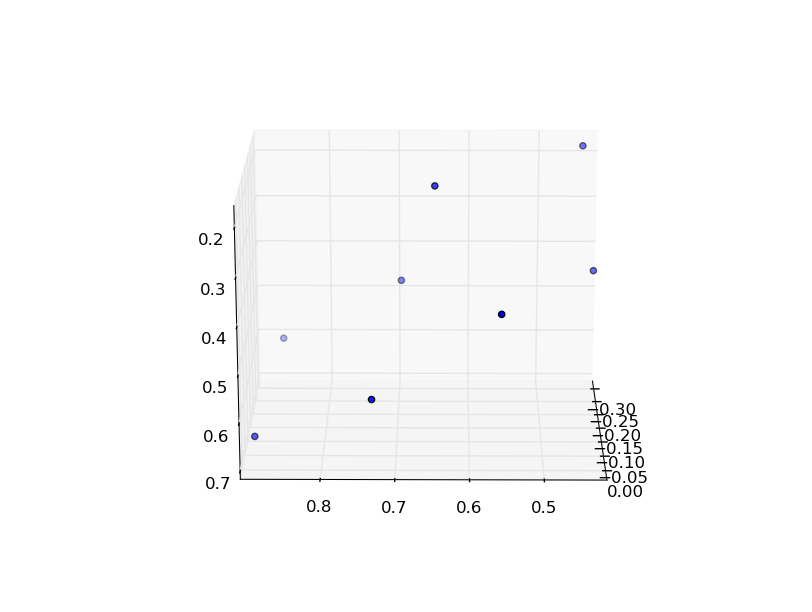
\includegraphics[width=0.8\linewidth,angle=0]{na4_4.png}
\caption{$Na_4Cl_4$ fourth configuration}
\label{figure7}
\end{center}
\end{figure}

Fifth one ~\ref{figure8}, with binding energy -6.680eV

\begin{figure}
\begin{center}
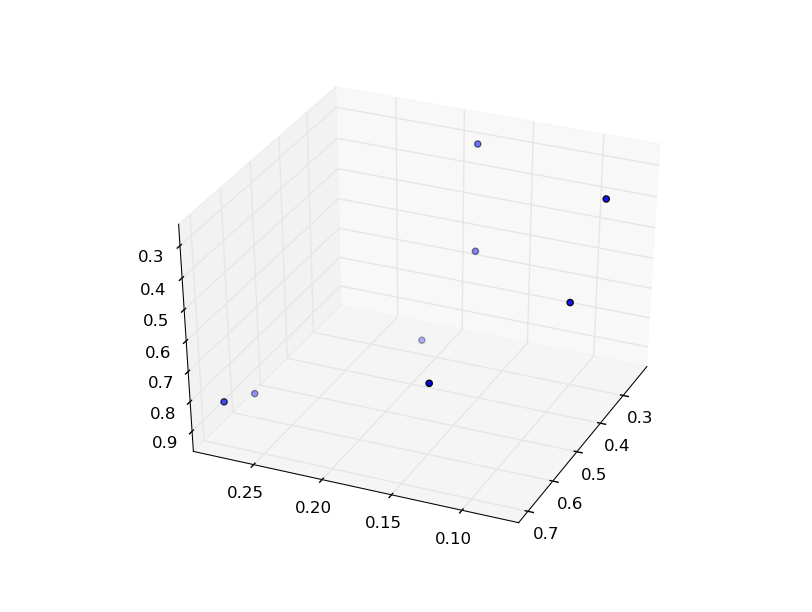
\includegraphics[width=0.8\linewidth,angle=0]{na4_5.png}
\caption{$Na_4Cl_4$ fifth configuration}
\label{figure8}
\end{center}
\end{figure}

It took me a lot of time to find the right configuration. For in our program precision is a finite number, in fact, big enough to cause problems. Considering the whole procedure, when the difference is within the defined precision program assumes it's the right configuration, however, it is under lots of situations not the local minima, in these cases, the configurations are either distorted "right" configurations or meaningless. Despite I used random initial guess, still it's with some certain pattern, thus some configurations are quite difficult to reach. I managed to finally get all configurations in the reference by making guess with certain constrains and giving smaller precision.

\newpage

\section{Problem 3}
\subsection{Description}
Download the NOAA Mauna Loa CO   data set (included in the lecture 6 and lecture 7 example code, if the link is not working) and modify thecode to generate graphs using other columns in the data. Does the average rate of increase depend on which colums are used in a straight line fit? Explore linear models with 3 terms to decide whether the linear rate of increase is accelerating or decelerating. If the current rate of increase continues indefinitely, when will the concentration become toxic (50,000 ppm)?

Repeat this exercise, but instead of a linear fit, implement a quadratic fit to the data :
$$
y=ax^2+bx+c
$$
Do this by minimizing the chi-squared function with BFGS or some other minimization algorithm. Compare to the simple matrix inversion fit of the linear problem as described in Lecture 14. 

\subsection{Result}
I used the BFGS method to perform the minimization of chi-squared function when applying quadratic fit to the CO2 data. However, this case is a little complicated for the following reasons:\\
First, if using the year directly, the numerical result for some steps will be too big, I consequently using the year-1953 as the x component
Additionally, even if I applied the year transform, considering it is large amount of data we are dealing with, and the default setting of BFGS method is to use an identity matrix for the first step, and our program in python do not support high enough precision, the minimization can fail under lots of circumstances. Therefore, I modified the program in two ways: one is before minimization, pick 3 points from the raw data and perform a Gauss-Jordan elimination to calculate a,b,c as the initial guess, so that the error can be small enough to continue iterations. Two, modified the $\sigma$ in the chi-squared function so that the error can be small enough for further iterations.\\
Though the second modification is not quite justified, considering the specific case we are using, the limitation of python, and it is one out of three problems of one of the all homework assignments of one of the many courses, although my favourite one. I would say it is a rather elegant solution, combining the knowledge I've learned with new tools. And the result looks also quite optimal. Here is the plots of both BFGS and poly fit ~\ref{figure9}  

\begin{figure}
\begin{center}
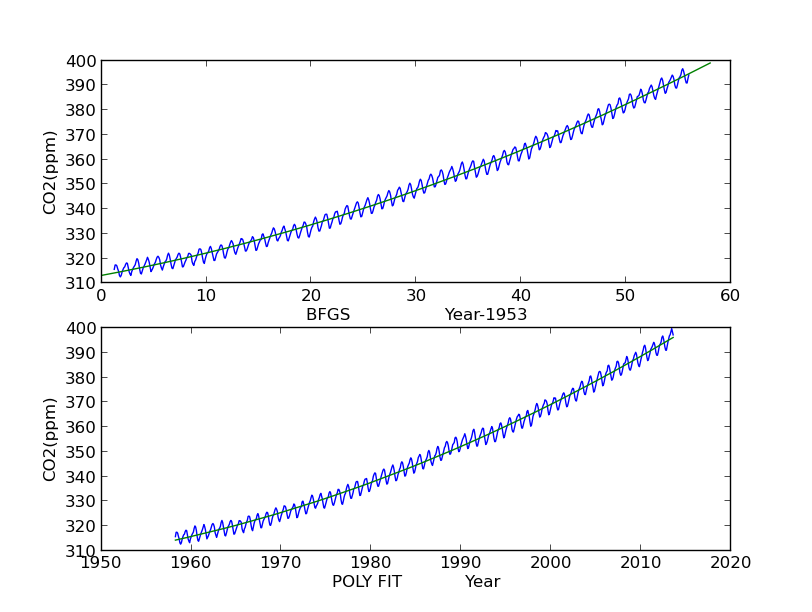
\includegraphics[width=0.8\linewidth,angle=0]{co2all.png}
\caption{CO2 fit with both BFGS and poly fit}
\label{figure9}
\end{center}
\end{figure}



\newpage
\section*{Acknowledgements}

I discussed this assignment with my classmates and used material from the
cited references, but this write-up is my own.

\begin{thebibliography}{9}


\bibitem{coursepage}
PHY 410-505 Webpage, \url{http://www.physics.buffalo.edu/phy410-505}.



\bibitem{paper}
Evolving few-ion clusters of Na and Cl 
\url{http://scitation.aip.org/content/aapt/journal/ajp/66/3/10.1119/1.18851}

\bibitem{plot of 2d function}
\url{http://www.wolframalpha.com/input/?i=plot+-0.5*%28x^2%2By^2%29%2B0.25*%28x^2%2By^2%29^2}

\end{thebibliography}

\newpage
\appendix
\section{Appendix}

\subsection{python code}

The following python code was used to obtain the results in this report:

\lstinputlisting[language=python]{minimize.py}

\lstinputlisting[language=python]{na3cl3.py}

\lstinputlisting[language=python]{co2chiminimize.py}

\end{document}
